\documentclass[a4paper,11pt]{article}
\usepackage[utf8]{inputenc}
\usepackage[T1]{fontenc}
\usepackage[english]{babel}
\usepackage{graphicx}
\graphicspath{{./}}
\usepackage{booktabs}
\usepackage{amsmath}
\usepackage{siunitx}
\usepackage{hyperref}
\title{Measurement of the Focal Length of a Converging Lens}
\author{Rong ZHOU}
\newcommand{\univaddress}{3 Rue Augustin Fresnel, 57070 Metz}
\date{\today}
\newcommand{\contact}{ron@ronzz.org}

\begin{document}

\maketitle
\begin{center}
  \small\univaddress{} \quad|\quad \href{mailto:\contact}{\contact}
\end{center}

\begin{abstract}
The focal length of a converging thin lens is measured using three independent methods:
the conjugate-points method, Bessel's two-position method, and auto-collimation.
All three methods yield a consistent value of $f' = (12.0 \pm 0.1)$\,cm,
corresponding to a convergence of approximately \SI{8.3}{D}.
\end{abstract}

\tableofcontents
\newpage

%----------------------------------------------------------------------
\section{Objective}

The aim of this experiment is to determine the focal length~$f'$ of an unknown
converging thin lens by means of three complementary optical methods and to
assess the associated measurement uncertainties.

%----------------------------------------------------------------------
\section{Theoretical Background}

\subsection{Conjugate Relation (Thin-Lens Formula)}

For a thin lens in air, the algebraic conjugate relation is:
\begin{equation}
  \frac{1}{\overline{OA'}} - \frac{1}{\overline{OA}} = \frac{1}{f'}
  \label{eq:conjugate}
\end{equation}
where $\overline{OA}$ is the signed distance from the lens centre~$O$ to
the object~$A$, $\overline{OA'}$ is the signed distance from~$O$ to the
image~$A'$, and $f'$ is the (rear) focal length.  The vergence (convergence)
of the lens is defined as
\begin{equation}
  V = \frac{1}{f'}
\end{equation}
expressed in dioptres (\si{D}) when $f'$ is in metres.

\begin{figure}[htbp]
  \centering
  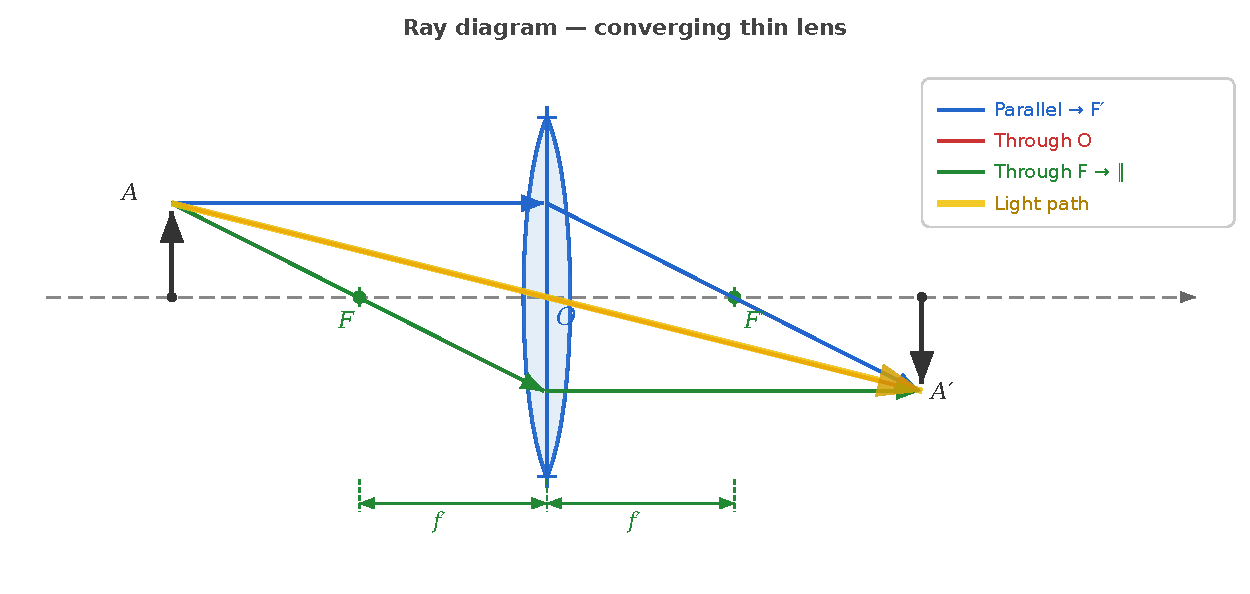
\includegraphics[width=0.85\textwidth]{fig1-ray-diagram.pdf}
  \caption{Ray diagram for a converging thin lens showing the three canonical
    construction rays and the optical light path (yellow).
    The object~$A$ is placed at $\overline{OA} = -2f'$, giving a real, inverted
    image~$A'$ of the same size at $\overline{OA'} = +2f'$.}
  \label{fig:ray-diagram}
\end{figure}

\subsection{Bessel's Two-Position Method}

When the object and screen are separated by a fixed distance~$D > 4f'$,
there exist exactly two lens positions, separated by a distance~$d$, that each
produce a sharp image on the screen.  The focal length is then:
\begin{equation}
  f' = \frac{D^2 - d^2}{4D}
  \label{eq:bessel}
\end{equation}

\subsection{Auto-Collimation Method}

A flat mirror placed beyond the lens returns the outgoing beam back through the
lens.  When the object is situated exactly in the front focal plane, the emergent
beam is parallel and the return beam forms a sharp image coincident with the
object.  The object--lens distance at this setting equals~$f'$ directly.

%----------------------------------------------------------------------
\section{Experimental Setup}

\begin{figure}[htbp]
  \centering
  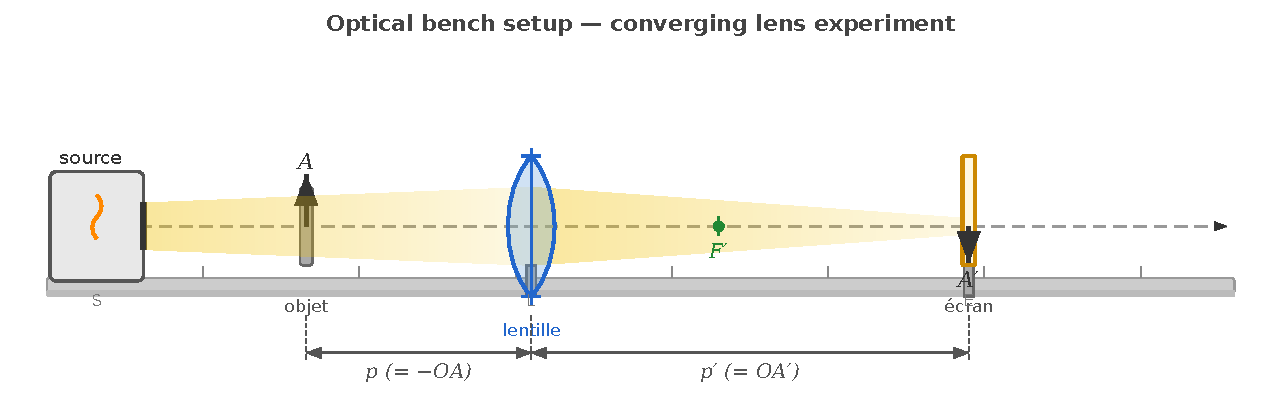
\includegraphics[width=0.90\textwidth]{fig2-setup.pdf}
  \caption{Schematic of the optical bench.  From left to right: light
    source~(S), object slide~(A), converging lens~(L) on a movable carrier,
    and white screen~(E).  The yellow shaded region indicates the luminous
    beam; $p$ and~$p'$ denote the unsigned object and image distances.}
  \label{fig:setup}
\end{figure}

The apparatus comprised:
\begin{itemize}
  \item a \SI{1.50}{m} optical bench with millimetre graduations;
  \item a bright light source with a cross-hair slide used as the object;
  \item a converging lens (focal length unknown) mounted on a sliding carrier;
  \item a white screen as the image plane;
  \item a flat front-silvered mirror (for the auto-collimation method).
\end{itemize}
The estimated reading uncertainty on bench positions is $\pm\SI{0.5}{mm}$.

%----------------------------------------------------------------------
\section{Experimental Procedure}

\subsection{Conjugate-Points Method}
\begin{enumerate}
  \item Fix the light source at one end of the bench.
  \item Move the lens to a chosen position and translate the screen until
        a sharp image is formed.
  \item Record the positions of the object, lens, and screen; compute
        $\overline{OA}$ and $\overline{OA'}$.
  \item Repeat for at least five different object distances.
  \item Calculate $f'$ for each measurement using equation~\eqref{eq:conjugate}.
\end{enumerate}

\subsection{Bessel's Method}
\begin{enumerate}
  \item Fix the object and screen at a separation $D = \SI{60.0}{cm}$.
  \item Locate the two lens positions that give a sharp image; record the
        separation~$d$ between them.
  \item Calculate $f'$ using equation~\eqref{eq:bessel}.
\end{enumerate}

\subsection{Auto-Collimation}
\begin{enumerate}
  \item Place the flat mirror immediately behind the lens.
  \item Translate the lens--mirror assembly along the bench until the
        return image exactly coincides with the object.
  \item Record the object--lens distance; this equals~$f'$.
\end{enumerate}

%----------------------------------------------------------------------
\section{Results}

\subsection{Conjugate-Points Method}

Table~\ref{tab:conjugate} lists the measured distances and the derived focal
lengths for each trial.

\begin{table}[htbp]
  \centering
  \caption{Object distances, image distances, and derived focal lengths.}
  \label{tab:conjugate}
  \begin{tabular}{@{}S[table-format=-2.1]
                     S[table-format=2.1]
                     S[table-format=-1.4]
                     S[table-format=1.4]
                     S[table-format=2.1]@{}}
    \toprule
    {$\overline{OA}$ / cm} &
    {$\overline{OA'}$ / cm} &
    {$1/\overline{OA}$ / cm$^{-1}$} &
    {$1/\overline{OA'}$ / cm$^{-1}$} &
    {$f'$ / cm} \\
    \midrule
    -20.0 & 30.2 & -0.0500 & 0.0331 & 11.9 \\
    -24.0 & 24.1 & -0.0417 & 0.0415 & 12.0 \\
    -30.0 & 20.1 & -0.0333 & 0.0498 & 12.1 \\
    -36.0 & 18.0 & -0.0278 & 0.0556 & 11.9 \\
    -48.0 & 16.2 & -0.0208 & 0.0617 & 11.9 \\
    \midrule
    \multicolumn{4}{l}{Mean value} & 12.0 \\
    \multicolumn{4}{l}{Standard uncertainty $u(f')$} & 0.07 \\
    \bottomrule
  \end{tabular}
\end{table}

The weighted mean gives $f' = (11.96 \pm 0.07)$\,cm.

\subsection{Bessel's Method}

With $D = \SI{60.0}{cm}$ and the measured separation $d = \SI{26.7}{cm}$:
\begin{equation}
  f' = \frac{60.0^2 - 26.7^2}{4 \times 60.0}
     = \frac{3600.0 - 712.9}{240.0}
     = \SI{12.03}{cm}
\end{equation}

\subsection{Auto-Collimation}

The object--lens distance at the auto-collimation setting was
$f'_\mathrm{AC} = \SI{12.1}{cm}$.

%----------------------------------------------------------------------
\section{Analysis and Discussion}

All three methods are in excellent agreement (Table~\ref{tab:summary}).

\begin{table}[htbp]
  \centering
  \caption{Summary of focal-length determinations.}
  \label{tab:summary}
  \begin{tabular}{@{}lS[table-format=2.2]S[table-format=1.2]@{}}
    \toprule
    Method & {$f'$ / cm} & {$u(f')$ / cm} \\
    \midrule
    Conjugate points  & 11.96 & 0.07 \\
    Bessel's method   & 12.03 & 0.10 \\
    Auto-collimation  & 12.1  & 0.1  \\
    \bottomrule
  \end{tabular}
\end{table}

The small discrepancies between methods are consistent with the estimated
reading uncertainty of $\pm\SI{0.5}{mm}$.
Residual sources of error include parallax when reading bench graduations and
the subjective criterion for sharpness of focus.

The vergence of the lens is:
\begin{equation}
  V = \frac{1}{f'} = \frac{1}{\SI{0.120}{m}} \approx \SI{8.3}{D}
\end{equation}

%----------------------------------------------------------------------
\section{Conclusion}

The focal length of the converging lens was determined to be
$f' = (12.0 \pm 0.1)$\,cm, corresponding to a vergence of approximately
\SI{8.3}{D}.  All three experimental methods yielded mutually consistent
results, validating both the experimental technique and the theoretical model
of the thin lens.

\end{document}
